%% REPLACE sXXXXXXX with your student number
\def\studentNumber{s1803764}


%% START of YOUR ANSWERS
%% Add answers to the questions below, by replacing the text inside the brackets {} for \youranswer{ "Text to be replaced with your answer." }. 
%
% Do not delete the commands for adding figures and tables. Instead fill in the missing values with your experiment results, and replace the images with your own respective figures.
%
% You can generally delete the placeholder text, such as for example the text "Question Figure 2 - Replace the images ..." 
%
% There are 19 TEXT QUESTIONS (a few of the short first ones have their answers added to both the Introduction and the Abstract). Replace the text inside the brackets of the command \youranswer with your answer to the question.
%
% There are also 3 "questions" to replace some placeholder FIGURES with your own, and 3 "questions" asking you to fill in the missing entries in the TABLES provided. 
%
% NOTE! that questions are ordered by the order of appearance of their answers in the text, and not by the order you should tackle them. Specifically, you cannot answer Questions 2, 3, and 4 before concluding all of the relevant experiments and analysis. Similarly, you should fill in the TABLES and FIGURES before discussing the results presented there. 
%
% NOTE! If for some reason you do not manage to produce results for some FIGURES and TABLES, then you can get partial marks by discussing your expectations of the results in the relevant TEXT QUESTIONS (for example Question 8 makes use of Table 1 and Figure 2).
%
% Please refer to the coursework specification for more details.


%% - - - - - - - - - - - - TEXT QUESTIONS - - - - - - - - - - - - 

%% Question 1: define overfitting
\newcommand{\questionOne} {
\youranswer{when a model learns the ”noise” in the training data and becomes too specific so that it does not do well when generalizing to new unseen data}
}

%% Question 2: Summarise the effect increasing width and depth of the architecture had on overfitting
\newcommand{\questionTwo} {
\youranswer{improves the validation accuracy but worsens the validation error, this indicates that our model is likely overfitting to certain samples in the training set and thus only similar samples in the validation set receive accurate classification }
}
%helps until the number of parameters becomes too high so that each layer just memorizes the training data, and you can end up with a neural network that fails to generalize well to new unseen data

%% Question 3: Summarise what your results show you about the effect of the tested approaches on overfitting and the performance of the trained model
\newcommand{\questionThree} {
\youranswer{dropout is a very effective technique for mitigating overfitting as it ensures that every node in the network takes on more responsibility for the inputs, for all combinations of hidden units and layers dropout always improved performance.} 
}

%% Question 4: Give your overall conclusions
\newcommand{\questionFour} {
\youranswer{Q4}
}

%% Question 5: Explain what overfitting is in detail and in your own words
\newcommand{\questionFive} {
\youranswer{the gap between the training error and test error is large as this indicates that the model learned the "noise" in the training data and thus is unable to generalize well to new unseen data such as the test set}
}

%% Question 6: Discuss ``why'' and ``how'' overfitting occurs, and ``how'' one can identify it is happening
\newcommand{\questionSix} {
\youranswer{Q6}
}

%% Question 7: Explain what these figures contain and how the curves evolve, and spot where overfitting occurs. Reason based on the min/max points and velocities (direction and magnitude of change) of the accuracy and error curves
\newcommand{\questionSeven} {
\youranswer{Q7}
}

%% Question 8: Explain your network width experiment results by using the relevant figure and table
\newcommand{\questionEight} {
\youranswer{Q8}
}

%% Question 9: Discuss whether varying width affects the results in a consistent way, and whether the results are expected and match well with the prior knowledge (by which we mean your expectations as are formed from the relevant Theory and literature)
\newcommand{\questionNine} {
\youranswer{Q9}
}

%% Question 10: Explain your network depth experiment results by using the relevant figure and table
\newcommand{\questionTen} {
\youranswer{Q10}
}

%% Question 11: Discuss whether varying depth affects the results in a consistent way, and whether the results are expected and match well with the prior knowledge (by which we mean your expectations as are formed from the relevant Theory and literature)
\newcommand{\questionEleven} {
\youranswer{Q11}
}

%% Question 12: Compare and discuss how varying width and height changes the performance and overfitting in your experiments
\newcommand{\questionTwelve} {
\youranswer{Q12}
}

%% Question 13: Explain L1/L2 weight penalties first in words and then with formulas. Explain how they are incorporated to training and what hyperparameter(s) they require
\newcommand{\questionThirteen} {
\youranswer{Q13}
}

%% Question 14: Discuss how/why the weight penalties may address overfitting, discuss how L1 and L2 regularization differ and support your claims with references where possible
\newcommand{\questionFourteen} {
\youranswer{Q14}
}

%% Question 15: Explain the experimental details (e.g. hyperparameters), discuss the results in terms of their generalization performance and overfitting
\newcommand{\questionFifteen} {
\youranswer{Q15}
}

%% Question 16: Explain the motivation behind Maxout Networks as presented in \cite{goodfellow2013maxout}
\newcommand{\questionSixteen} {
\youranswer{Q16
}
}

%% Question 17: State whether Dropout is compatible (can be used together) with Maxout and explain why
\newcommand{\questionSeventeen} {
\youranswer{Q17
}
}

%% Question 18: Give an overview of the experiment setup in \cite{goodfellow2013maxout} and analyse it from the point of view of how convincing their conclusions are 
\newcommand{\questionEighteen} {
\youranswer{Q18
}
}

%% Question 19: Briefly draw your conclusions based on the results from the previous sections (what are the take-away messages?) and conclude your report with a recommendation for future directions
\newcommand{\questionNineteen} {
\youranswer{Q19
}
}


%% - - - - - - - - - - - - FIGURES - - - - - - - - - - - - 

%% Question Figure 2:
\newcommand{\questionFigureTwo} {
\youranswer{Question Figure 2 - Replace the images in Figure 2 with figures depicting the accuracy and error, training and validation curves for your experiments varying the number of hidden units.
%
\begin{figure}[t]
    \centering
    \begin{subfigure}{\linewidth}
        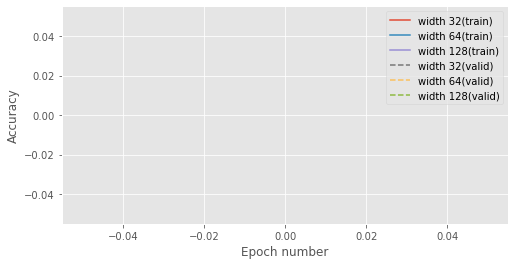
\includegraphics[width=\linewidth]{figures/empty_acc_curve_width.png}
        \caption{accuracy by epoch}
        \label{fig:width_acccurves}
    \end{subfigure} 
    \begin{subfigure}{\linewidth}
        \centering
        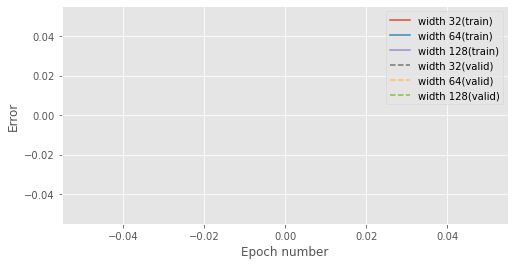
\includegraphics[width=\linewidth]{figures/empty_error_curve_width.png}
        \caption{error by epoch}
        \label{fig:width_errorcurves}
    \end{subfigure} 
    \caption{Training and validation curves in terms of classification accuracy (a) and cross-entropy error (b) on the EMNIST dataset for different network widths.}
    \label{fig:width}
\end{figure} 
}
}

%% Question Figure 3:
\newcommand{\questionFigureThree} {
\youranswer{Question Figure 3 - Replace these images with figures depicting the accuracy and error, training and validation curves for your experiments varying the number of hidden layers.
%
\begin{figure}[t]
    \centering
    \begin{subfigure}{\linewidth}
        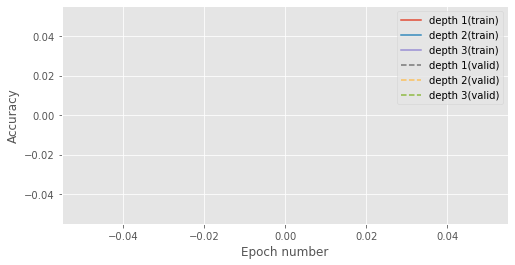
\includegraphics[width=\linewidth]{figures/empty_acc_curve_depth.png}
        \caption{accuracy by epoch}
        \label{fig:depth_acccurves}
    \end{subfigure} 
    \begin{subfigure}{\linewidth}
        \centering
        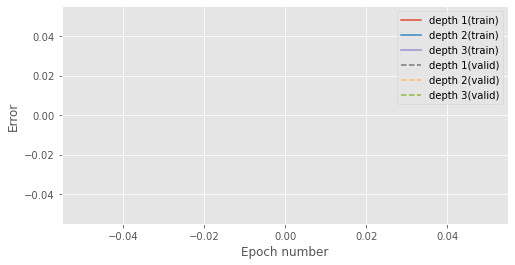
\includegraphics[width=\linewidth]{figures/empty_error_curve_depth.png}
        \caption{error by epoch}
        \label{fig:depth_errorcurves}
    \end{subfigure} 
    \caption{Training and validation curves in terms of classification accuracy (a) and cross-entropy error (b) on the EMNIST dataset for different network depths.}
    \label{fig:depth}
\end{figure} 
}
}

%% Question Figure 4:
\newcommand{\questionFigureFour} {
\youranswer{Question Figure 4 - Replace these images with figures depicting the Validation Accuracy and Generalisation Gap for each of your experiments varying the Dropout inclusion rate, L1/L2 weight penalty, and for the 8 combined experiments (you will have to find a way to best display this information in one subfigure).
%
\begin{figure*}[t]
    \centering
    \begin{subfigure}{.3\linewidth}
        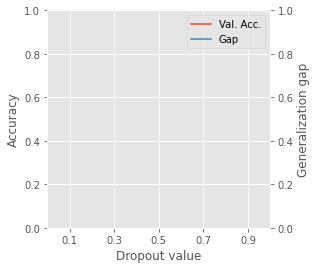
\includegraphics[width=\linewidth]{figures/empty_dropout_plot.png}
        \caption{Metrics by inclusion rate}
        \label{fig:dropoutrates}
    \end{subfigure} 
    \begin{subfigure}{.3\linewidth}
        \centering
        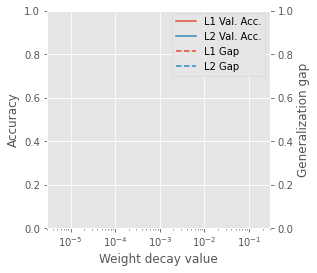
\includegraphics[width=\linewidth]{figures/empty_wd_plot.png}
        \caption{Metrics by weight penalty}
        \label{fig:weightrates}
    \end{subfigure} 
    \begin{subfigure}{.3\linewidth}
        \centering
        \includegraphics[width=.85\linewidth]{example-image-duck}
        \caption{Extra experiments}
        \label{fig:extra}
    \end{subfigure} 
    \caption{Hyperparameter search for every method and combinations}
    \label{fig:hp_search}
\end{figure*}
}
}

%% - - - - - - - - - - - - TABLES - - - - - - - - - - - - 

%% Question Table 1:
\newcommand{\questionTableOne} {
\youranswer{
Question Table 1 - Fill in Table 1 with the results from your experiments varying the number of hidden units.
%
\begin{table}[t]
    \centering
    \begin{tabular}{c|cc}
    \toprule
        \# hidden units & val. acc. & generalization gap \\
    \midrule
         32            &            &                    \\
         64            &            &                    \\
         128           &            &                    \\ 
    \bottomrule
    \end{tabular}
    \caption{Validation accuracy (\%) and generalization gap (in terms of cross-entropy error) for varying network widths on the EMNIST dataset.}
    \label{tab:width_exp}
\end{table}
}
}

%% Question Table 2:
\newcommand{\questionTableTwo} {
\youranswer{
Question Table 2 - Fill in Table 2 with the results from your experiments varying the number of hidden layers.
%
\begin{table}[t]
    \centering
    \begin{tabular}{c|cc}
    \toprule
        \# hidden layers & val. acc. & generalization gap \\
    \midrule
         1               &            &                    \\
         2               &            &                    \\
         3               &            &                    \\ 
    \bottomrule
    \end{tabular}
    \caption{Validation accuracy (\%) and generalization gap (in terms of cross-entropy error) for varying network depths on the EMNIST dataset.}
    \label{tab:depth_exps}
\end{table}
}
}

%% Question Table 3:
\newcommand{\questionTableThree} {
\youranswer{
Question Table 3 - Fill in Table 3 with the results from your experiments varying the hyperparameter values for each of L1 regularisation, L2 regularisation, and Dropout (use the values shown on the table) as well as the results for your experiments combining L1/L2 and Dropout (you will have to pick what combinations of hyperparameter values to test for the combined experiments; each of the combined experiments will need to use Dropout and either L1 or L2 regularisation; run an experiment for each of 8 different combinations). Use \textit{italics} to print the best result per criterion for each set of experiments, and \textbf{bold} for the overall best result per criterion.
%
\begin{table*}[t]
    \centering
    \begin{tabular}{c|c|cc}
    \toprule
        Model    &  Hyperparameter value(s) & Validation accuracy & Generalization gap \\
    \midrule
    \midrule
        Baseline &  -                    &               0.836 &                 0.290 \\
    \midrule
        \multirow{3}*{Dropout}
                 & 0.7                   &                     &                   \\
                 & 0.9                   &                     &                   \\
                 & 0.95                  &                     &                   \\
    \midrule
        \multirow{3}*{L1 penalty}
                 & 1e-4                   &                     &                   \\
                 & 1e-3                   &                     &                   \\
                 & 1e-1                   &                     &                   \\
    \midrule
        \multirow{3}*{L2 penalty}  
                 & 1e-4                   &                     &                   \\
                 & 1e-3                   &                     &                   \\
                 & 1e-1                   &                     &                   \\
    \midrule
        \multirow{6}*{Combined}  
                 & for example 0.95, L1 1e-6  &                     &                   \\
                 & ?, ?                   &                     &                   \\
                 & ?, ?                   &                     &                   \\
                 & ?, ?                   &                     &                   \\
                 & ?, ?                   &                     &                   \\
                 & ?, ?                   &                     &                   \\
    \bottomrule
    \end{tabular}
    \caption{Results of all hyperparameter search experiments. \emph{italics} indicate the best results per series and \textbf{bold} indicate the best overall}
    \label{tab:hp_search}
\end{table*}
}
}

%% END of YOUR ANSWERS